\newtheorem{definition}{\textbf{Definice}}

\chapter{Úvod}
\label{ch:uvod}



V~dnešní době, je obor umělé inteligence (AI), postupem let všudypřítomnější a její působení ovlivňuje spoustu aspektů našeho života.

Pokrok umělé inteligence je dobře měřitelný jejím aplikováním v~oblasti her.
A~to proto, že právě hry nabízí jasně definovaná pravidla a cíle, čímž se stávají ideálním testovacím prostorem pro algoritmy umělé inteligence.
Výkon AI je ve hrách snadno měřitelný a pokrok dokáže vidět i laik bez žádných složitých grafů, tabulek a výpočtů.
Umělá inteligence již dokázala porazit nejlepší hráče v~\textit{šachu}~\cite{DeepBlue}, \textit{Dota 2}~\cite{Dota2}, \textit{Go}~\cite{AlphaGo} a spoustě dalších her.

Hra studovaná v~této práci se jmenuje \emph{Scotland Yard}.
Jedná se o~hru pro tři až šest hráčů.
V~této hře obvykle hraje jeden hráč jako Pan~X, který se snaží uniknout policistům, ovládanými ostatními hráči.
Policisté, avšak nevědí, kde na herním poli se Pan~X nachází.
A~musí tedy odhadovat jeho pozici a spolupracovat mezi sebou, aby ho mohli polapit.
Pozice Pana~X je policistům odhalena pouze v~určitých kolech.
Scotland Yard je ideální hrou ke studování neurčitosti ve hrách hranými systémy umělé inteligence, protože se jedná o~hru s~nedokonalou informací a k~vítězství policistů je zapotřebí spolupráce, strategie a odhadování neznámé informace.

Tato práce zkoumá algoritmy posilovaného učení, jejich použití na hry s~neurčitostí a jejich porovnání s~klasickými metodami hraní her.
Algoritmus optimalizace proximální strategie (Proximal Policy Optimization--PPO) je hlavním zkoumaným algoritmem této práce.
PPO je často používán k~řešení problémů se spojitými veličinami a ve 3D prostoru.
Pro srovnání s~jinými algoritmy slouží algoritmus Deep--Q--Learning (DQN).
Výslední agenti\footnote[1]{V kontextu se hrou Scotland Yard je důležité nezaměňovat agenta, za policistu. Význam pojmu \emph{agent} je popsáno v kapitole \nameref{subsec:agent}} byli také testování proti hráči, který náhodně vybírá své akce.

Algoritmus PPO byl vybrán z~důvodu jeho úspěšnosti při použití ve složitých hrách s~neurčitostí.
Tyto tvrzení podporuje experiment OpenAI~\cite{PPO_Hide_Seek_page}, podrobně popsán zde~\cite{PPO_Hide_Seek_paper}.
V~tomto experimentu byla optimalizace proximální strategie použita pro učení strategie ve hře typu \textit{schovávaná} s~několika agenty a neúplnou informací.
Jelikož tento typ hry přesně odpovídá i hře Scotland Yard, zdá se být vhodný i pro řešení této hry.
Také další studie~\cite{Manille} a~\cite{Dota2} tento výrok dále podporují a dokazují vhodnost algoritmu PPO pro tuto práci.

Zaměření této práce jsem si vybral, jelikož mi vždy byl obor umělé inteligence blízký a vždy jsem se chtěl začít tomuto odvětví více věnovat i po praktické stránce.
Algoritmus je pro mě zajímavý a zkušenost s~tímto algoritmem by se dala využít v~mém dalším pracovním životě.\newpage

Pro zpracování práce byly využity tyto hlavní knihovny:
\begin{itemize}
  \item \texttt{Ray.Rlib} - framework pro posilované učení. Obsahuje již zhotovenou implementací algoritmu PPO a DQN, které byly použity v~této práci. 
  \item \texttt{PyTorch} - podpůrná knihovna \texttt{Ray.Rlib}
  \item \texttt{Gymnasium} - knihovna použita k~vytvoření prostředí hry Scotland Yard
  \item \texttt{Pygame} - knihovna pro vytváření uživatelského rozhraní
\end{itemize}

Práce byla zhotovena pro operační systémy Windows a Python verze 3.10

\chapter{Teoretický základ}
\label{ch:teoreticky_zaklad}
Tato kapitola není encyklopedickým přehledem celého tématu bakalářské práce.
Nýbrž jedná se o~shrnutí nejdůležitějších relevantních informací a pojmů, důležitých pro tuto práci.

\section{Desková hra Scotland Yard}
\label{sec:deskova-hra-scotland-yard}

Scotland Yard je populární hra pro tři a více hráčů, která kombinuje prvky schovávané a hry na honěnou.
Jeden hráč hraje za Pana~X, který se snaží uniknout policistům a ti jsou ovládáni zbylými hráči.
Hra je u~konce, pakliže je Pan~X úspěšně chycen policisty (vyhrávají policisté), nebo když je dosažen maximální počet kol, bez toho aniž by byl Pan X chycen (vyhrává Pan~X).
Originální hra se odehrává na mapě Londýna.

\begin{figure}[H]
	\centering
	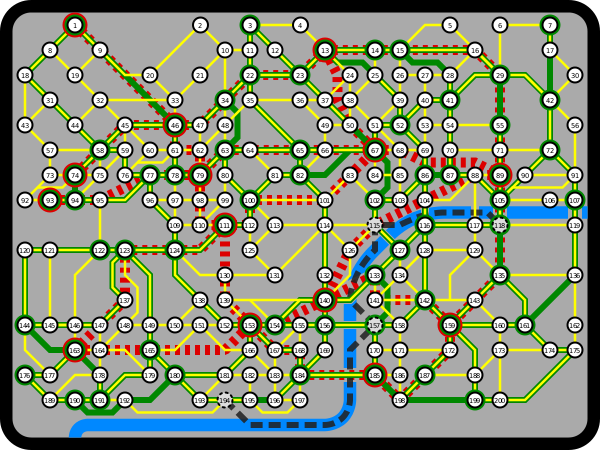
\includegraphics[width=0.87\textwidth]{obrazky-figures/scotland_original}
	\caption{Ukázka herní mapy hry Scotland Yard.
  Zdroj~\cite{scotland_original_image}:}\label{fig:figure}
\end{figure}
\newpage

Na této herní mapě nachází 200 polí, které jsou vzájemně propojené cestami.
Každá z~těchto cest povoluje pouze určitý způsob dopravy (např. pouze taxíkem, pouze autobusem atd.).
Jednotliví hráči využívají prvky veřejné dopravy k~pohybu po herní ploše, kterými jsou:

\begin{itemize}\vspace{-0.3cm}
  \item \emph{Taxi}\vspace{-0.3cm}
  \item \emph{Autobus}\vspace{-0.3cm}
  \item \emph{Metro}\vspace{-0.3cm}
  \item \emph{Trajekt}
\end{itemize}

Každému hráči je na začátku hry přidělen pouze určitý počet jízdenek na tyto typy dopravních prostředků.
K~využití dopravy je použita právě tato jízdenka.
Pokud již hráč nemá některou z~typů jízdenek, nemůže nadále tento způsob přepravy využívat.
Hra se dělí na kola, ve kterých se hráči postupně střídají.
Jakmile Pan X provede svůj tah, je odhaleno pouze jaký typ dopravy využil, ale neodhaluje na které místo se přemístil.

Hlavní myšlenkou hry je, že po většinu kol je pozice Pana~X policistům utajena.
Odhaluje se jim pouze určená kola.
To znamená, že policisté pro polapení Pana~X musí odhadovat jeho pozici a spolupracovat mezi sebou.
Tímto se ze hry Scotland Yard stává hra s~nedokonalou informací, jelikož policisté nevidí přesnou pozici Pana~X\@.
Tento fakt ji činí vhodnou pro studování metod hraní her s~neurčitostí.

Pan X má také možnost použít speciální akci, kterou je \emph{dvojitý tah}.
Také vlastní speciální jízdenku, která mu umožňuje použít jakýkoliv druh dopravy
Pokud Pan X použije tutu speciální jízdenku, není policistům odhalen jaký typ dopravy využil.

\section{Další hry s~nedokonalou informací a systémy využívající algoritmus PPO}\label{sec:dalsi-hry-s-nedokonalou-informaci}
V~oblasti umělé inteligence hraje důležitou roli modelování a řešení her.
Hry představují formalizaci konfliktních interakcí mezi aktéry.
Klasická teorie her se zaměřuje na hry s~úplnou informací, kde mají všechny strany v~daném okamžiku přístup ke všem relevantním informacím z~herního prostředí.
Znají strategie a cíle ostatních hráčů.
V~praxi se však častěji setkáváme se situacemi, kde jednotlivým stranám chybí některé informace, ať už se jedná o~informace z~prostředí či cíli soupeře.

Následující hry byly vybrány pro svou složitost a neúplnou informaci, kterou obsahují.
V obou případech byly prokázány dobré výsledky s použitím algoritmu PPO.
Na základě těchto výsledků i já zvolil algoritmus PPO pro řešení hry Scotland Yard.

\subsection{Dota 2}\label{subsec:dota}
Dota 2 je velmi komplexní strategická hra v~odehrávající se v~reálném čase.
Hraje se ve dvou týmech po pěti hráčích kteří ovládají postavy s~různými unikátními schopnostmi.
Schopnosti jsou hlavní součástí hry.
Díky schopnostem mohou hrdinové zranit nepřítele, udělat silnější sebe či své spojence a mohou mít i spousty dalších efektů.
Co jim navíc přidává na komplexnosti je to, že každá schopnost nemůže být po použití znovu použita po určitou dobu.
Zlato používají hráči jako herní měnu, za kterou si hrdinové mohou koupit různé předměty, které je posílí.

Ve hře se vyskytuje válečná mlha, která způsobuje že hráči vidí pouze část mapy ve svém okolí a okolí spřátelených jednotek.
To znamená, že hráči nemají úplnou informaci o~pozici nepřátelských jednotek.

\bigskip

Dota 2 je pro umělou inteligenci náročnou výzvou z~těchto důvodů:
\begin{itemize}
  \item Složitost hry

  Její stav se mění velmi rychle a je tedy těžké předpovídat vývoj hry.
  Agenti tedy musí být schopni rychle reagovat na změny a přizpůsobit svoji strategii.

  Pozorovací prostor je obrovský, obsahuje až 16 000 vstupů.
  Akční prostor je složitý, jelikož lidé hrají Dotu 2 většinou pomocí myši a klávesnice.
  U~OpenAI Five je akční prostor rozdělen na hlavní akce a parametry těchto akcí.
  Hlavní akce jsou například, pohyb, útok, použití schopnosti/ předmětu, zakoupení předmětu a další situační akce.
  Dostupnost těchto akcí je závislá na stavu hry a je řízena maskou akcí.
  Tyto akce mají 3 parametry, zpoždění, vybranou jednotku a offset cíle akce.
  Pokud tyto akce a jejich parametry zkombinujeme získáme akční prostor o~velikosti 1,837,080 dimenzí.

  \item Nedokonalá informace

  Právě kvůli válečné mlze nemají hráči úplnou informaci o~pozici nepřátelských jednotek a musí tedy pouze odhadovat kde na mapě se nachází.
  Neznají ani jestli jsou nepřátelé schopni použít své schopnosti a předměty.
  Ve hře dota 2 vykonávají hráči několik rozhodnutí někdy i několikrát za sekundu.
\end{itemize}

Dota 2 sama o~sobě obsahuje implementaci chování inteligentních agentů, kteří jsou schopni hrát hru na velmi vysoké úrovni.
Jejich výkon však není dostatečný a nebyli schopni ani zdaleka porazit zkušené.
Použité metody pro vytvoření těchto agentů bohužel nejsou zveřejněny.

Inovaci umělé inteligence v~této hře opět přinesla společnost OpenAI a jejich projekt \emph{OpenAI Five}~\cite{Dota2}.
Tento projekt se zaměřil na vytvoření modelu, který by byl schopen porazit nejlepší hráče světa ve hře Dota 2.
OpenAi zvolila pro učení výsledného modelu algoritmus \textbf{PPO}.
Agent OpenAI Five byl, kombinovaně s~předchozí verzí, trénován asi \emph{55 000} herních let hraním sama proti sobě.

I přes velikost hry je výsledný reakční čas agenta okolo 33ms, oproti tomu reakční čas profesionálních hráčů her je okolo 120ms~\cite{reaction_time}
OpenAi Five porazil tehdejší nejlepší tým světa během exhibice na nejprestižnějším turnaji Dota2 \textit{The International}.
V~celém exhibičním turnaji proti nejlepším týmům světa z~celkových 24 her vyhrál 19 her a pouhých 5 prohrál.

\subsection{Experiment OpenAI}\label{subsec:experiment-openai}
Důležitým zdrojem pro tuto práci byla studie~\cite{PPO_Hide_Seek_paper}, od společnosti OpenAI.
Z~ní vyplývá, že algoritmus \textbf{PPO} je vhodný pro řešení problémů s~nedokonalou informací.
V~dané studii byl algoritmus implementován na komplexní hru typu schovávaná.
Ve hře proti sobě hrají dva typy hráčů.
Modří hráči se snaží schovat a utéct před červenými.
Po herní ploše byly rozestavěny objekty, se kterými hráči mohou interagovat.
Mohou je přesouvat a následně \uv{zamrazit} na místě, takže s~objektem nelze pohybovat.
Modří hráči se na začátku hry objevují ve své pevnosti, která má několik děr.
Červeným hráčům je na začátku hry znemožněn pohyb, což dává modrým hráčům čas připravit se na jejich útok.

Po více než 8 miliónech epizodách učení se modří hráči naučili efektivně blokovat vstup do jejich pevnosti, takže je červení hráči nebyli schopni dostihnout.
Červení hráči se poté adaptovali a naučili se využívat rampy a přelézt opevnění modrých hráčů.
Finální strategii se modří naučili po 43 miliónech epizodách.
Modří hráči na začátku kola ukradli červeným všechny rampy a zabarikádovali se i s~nimi v~pevnosti.
Červení hráči tak neměli žádnou šanci na výhru.

Dokonce se objevili i fascinující strategie které zneužívaly chyby v~prostředí.
Například, v~kódu obsluhující kolize byla chyba, která způsobovala, že při najetí rampy na zeď arény, pod určitým úhlem, byla rampa rapidní rychlostí vymrštěna do vzduchu.
Toho červení hráči zneužili a za pomocí této chyby se vymršťovali do vzduchu, aby překonali zdi pevnosti modrých.


\section{Klíčové koncepty posilovaného učení}\label{sec:klicove-koncepty-posilovaneho-uceni}
Posilované učení (Reinforcement Learning, RL) je oblast strojového učení, která se zaměřuje na učení agentů v~dynamickém prostředí.
Agent se učí strategii chování, která maximalizuje kumulativní odměnu.

\subsection{Agent}\label{subsec:agent}
Je komplexní entita, která interaguje s~prostředím.
Prostředí poskytuje agentovi informace o~stavu a agent na základě těchto pozorování vykonává akce.
Tyto akce mohou ovlivnit stav prostředí a agent obdrží odměnu na základě odměnové funkce.
Agent většinou volí takové akce, aby maximalizoval kumulativní odměnu.

Pro textový obsah této práce je velmi důležité definovat pojem \emph{agent}.
Slovo je podobné slovu \emph{policista} a v kontextu hry Scotland Yard je tedy možné tyto významy zaměnit.\\
\emph{Slovo agent, v této práci výhradně značí entitu, která je zde byla popsána a nikde nevystupuje jako synonymum k policistům.}

\subsection{Pozorovací a akční prostor}
\label{subsec:prostory}

\textbf{Pozorovací prostor} je jednou z~nejdůležitějších součástí posilovaného učení.
Bez jeho vhodného zvolení, je dosažení strategie s~dobrými výsledky velmi obtížné.
Pozorovací prostor je množina všech možných pozorování, které může agent získat z~prostředí.
Je to tedy forma, kterou prostředí předává informace agentovi.
Velmi často se aktuální stav pozorovacího prostoru využívá jako stav.
Při vytváření prostředí je nutné definovat typ, tvar prostoru a jakých hodnot může nabývat.

Pro jeho podoby je vhodné zvolit standard z~knihovny \texttt{Gymnasium}~\cite{Gymnasium}.
Gymnasium je pokračování knihovny \texttt{Gym} od společnosti OpenAI\@.
Tyto knihovny nastavily standard vytváření prostředí pro posilované učení.
Dodržování těchto standardů umožňuje použití libovolného algoritmu na jedno prostředí.

\bigskip

\textbf{Akční prostor} je, jak název vypovídá, množina všech možných akcí, ze kterých může strategie volit.
Často se jedná o~konečnou množinu celočíselných hodnot, které reprezentují různé akce.
Samozřejmě může být akční prostor i spojitého typu (blíže popsáno v~další sekci).

V~herním prostředí mohou nastat situace kdy se nějaká akce stane nevalidní, jelikož by její provedení vyústilo v~nevalidní stav herního prostředí.
V~takovém případě je vhodné zvolení této akce zamezit, nejlépe pomocí akční masky.
Ta definuje, které akce jsou v~momentálním stavu prostředí proveditelné.
Lze také tyto akce povolit, ale následně agentovi udělit sníženou odměnu za provedení nevalidní akce.

\subsection{Diskrétní a spojitý prostor}\label{subsec:diskretni-a-spojity-prostor}

Je--li prostor o~\textbf{diskrétní}, je konečný nebo spočítatelně nekonečný. 
Příkladem takového prostoru je například pozorovací prostor, jehož vstupem je fotka.
Ta se dělí na přesně daný počet pixelů, kde každý má dané hodnoty RGB.
Diskrétní akční prostory jsou počítatelné a často se jedná o~konečnou množinu možných akcí.
Například akce pohybu \textit{vlevo}, \textit{vpravo}, \textit{nahoru}, \textit{dolů}.

Zato \textbf{spojitý prostor} je nekonečný a nespočítatelný. 
Spojitý pozorovací prostor je například pozice robota ve 3D prostoru, nebo jeho rychlost.
Spojitý akční prostor může například ovládat sílu stlačení pedálu, nebo úhel natočení kola.

\subsection{Prostředí}\label{subsec:prostredi2}

Je vše s~čím agent interaguje.
Prostředí je buď fyzické (entity z~reálného světa, ovládání chytré domácnosti, robotické ruky, ovládání reaktoru apod.) nebo virtuální (simulace nebo hra).
Prostředí reaguje na zvolené akce agenta poskytuje mu zpětnou vazbu ve formě odměny.
Odměna může být i záporná, pokud agent zvolil velmi nevhodnou akci.
Pokud v~prostředí existuje více agentů, může mít každý agent jiné pozorování.
Díky tomuto můžeme například schovat agentovi \textit{A} určité informace, které agent \textit{B} vidí.

\subsection{Strategie (Policy)}\label{subsec:strategie}

Pomocí posilovaného učení vzniká strategie.
Strategie je matematická funkce, která definuje agentovo chování na základě jeho pozorování (stavu).
Snaží se definovat takové chování, které vede k~maximální kumulativní odměně.
Strategie může být deterministická nebo stochastická.

  \subsubsection*{Deterministická strategie}
  
  Deterministická strategie přesně definuje cílový stav přechodu pro každý stav.
  Agent tedy pro jeden stav vždy volí stejnou akci.
  Tato strategie je vhodná, pokud je zapotřebí v~každém stavu reagovat konzistentně, bez odchylek.
  Například, pokud agent ovládá termostat v~domě a teplota je pod požadovanou hladinu.
  Nemůže se stát, aby byla šance, že agent zvolí akci, která teplotu ještě sníží.
  Další výhoda, je že je jednoduchá na interpretaci a implementaci~\cite{Policies}.

  Rovnice výsledné akce deterministické strategie je:
  \begin{equation}
    \pi(s) = a\label{eq:policy_deterministic}
  \end{equation}

  \subsubsection*{Stochastická strategie}
  
  Zato stochastická strategie definuje pro každý stav pravděpodobnostní rozdělení nad množinou akcí.
  Výsledná akce je tedy náhodná dle rozdělení pravděpodobnosti.
  Může tedy nastat situace kdy ve stejném stavu agent zvolí vždy jinou akci.
  Tato strategie je vhodná v~situacích, kdy je potřeba zkoumat různé strategie a kdy agent nemá úplnou informaci o~prostředí.
  Například tam kde by deterministická strategie zvolila jasnou akci \textit{A}, stochastická strategie by mohla s~malou pravděpodobností zvolit akci \textit{B}.
  Čímž ale může odhalit, že akce \textit{B} je s~ohledem na komulativní odměnu lepší než akce \textit{A}~\cite{Policies}.

  Rovnice výsledné akce stochastické strategie je:
  \begin{equation}
    \pi(a \vert s) = \mathbb{P}_\pi [A=a \vert S=s]\label{eq:policy_stochastic}
  \end{equation}

\subsection{Akce}\label{subsec:akce}

Akce je aktivita, proces či funkce kterou agent vykoná ve specifickém stavu~\cite{ActionCo67}.
Výsledkem provedení akce je tedy změna z~aktuálního stavu, do jiného, či stejného stavu z~množiny možných stavů.
Zjednodušeně, je to rozhodnutí, které agent vykonává v~prostředí a toto rozhodnutí ovlivňuje prostředí.

Akce může být také nedeterministická či stochastická.
Výsledný stav tedy může být jiný pro stejný stav a akci.
  
\subsection{Odměna}\label{subsec:odmena}

  Odměna je hodnota, kterou agent obdrží od prostředí po vybrání akce.
  Může být kladná, záporná nebo nulová.
  Dle této zpětné vazby se agent učí, jak moc byla jeho zvolená akce v~daném stavu vhodná.

\subsection{Hodnotová funkce}\label{subsec:hodnotova-funkce}

  Hodnotová funkce vyhodnocuje, jak dobrý je stav tím, že predikuje budoucí odměnu, pokud bude další tah začínat v~tomto stavu.
  Čím vzdálenější odměna je od tohoto stavu, tím více je snížena.
  Protože, čím je odměna vzdálenější tím více je nejisté, že bude doopravdy získána.

  Existují dva typy hodnotových funkcí:

  \subsubsection*{Hodnotová funkce stavu $V(s)$}

  Hodnotová funkce stavu \emph{$V(s)$} vyhodnocuje očekávanou komulativní odměnu, jestliže se agent nachází v~tomto stavu.
  Vyhodnocuje tedy jak příznivý je daný stav pro agenta.

  \subsubsection*{Hodnotová funkce akce $Q(s, a)$}
  \label{subsubsec:q_function}

  Hodnotová funkce akce \emph{$Q(s, a)$} vyhodnocuje očekávanou komulativní odměnu, pokud se agent nachází v~tomto stavu a zvolí tuto akci.
  Vyhodnocuje tedy jak dobré či špatné je zvolení dané akce v~aktuálním stavu.

\pagebreak

\subsection{Markovův rozhodovací proces}\label{subsec:markovovy-rozhodovaci-proces}

Téměř všechny problémy, řešené posilovaným učením, mohou být označeny jako Markovy rozhodovací procesy (Markov Decision Process).
Tato abstrakce je základním kamenem pro modelování algoritmů posilovaného učení.
Markovův rozhodovací proces značí, že následující stav není závislý na stavech minulých, nýbrž pouze na aktuálním stavu.

\begin{figure}[H]
	\centering
	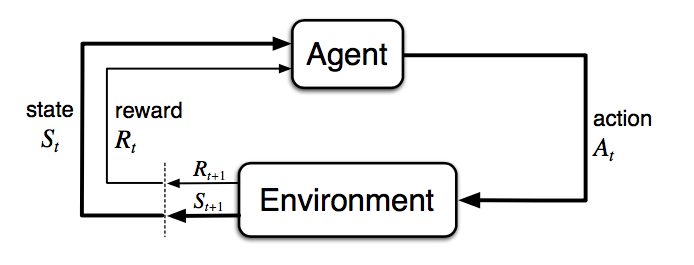
\includegraphics[width=0.6\textwidth]{obrazky-figures/RL_basics}
	\caption{Interakce mezi prostředím a agentem podle Markova rozhodovacího procesu.
  Zdroj~\cite{RL_basics}:}\label{fig:markov}
\end{figure}
\begin{definition}
\end{definition}

\subsection{Rovnováha mezi explorací a exploatací}
\label{subsec:exploration-exploitation-dillemma}
\begin{quote}
  \emph{Kompromis mezi potřebou získávat nové znalosti a potřebou použít již nabyté znalosti k~vylepšení výkonnosti je jedním z~nejzákladnějších kompromisů v~přírodě~\cite{Exploitation_Exploration}.}
\end{quote}
Explorace a exploatace jsou dvě protichůdné strategie, které se vyskytují jak ve strojovém učení, tak i v~reálném životě.

\emph{Exploatace} se snaží vybrat nejlepší možnou akci na bázi známých informací.
Tyto informace, nemusí být kompletní, nebo mohou být zavádějící.
A~to z~důvodu nedostatečného trénování, či nedostatečného prozkoumávání možností prostředí.

Tomu opačná metoda \emph{explorace} usiluje o~prozkoumání možností, které nejsou známé a mohly by vést k~lepší budoucí odměně.
Explorace tedy často zvolí akci, která nemusí být nejlepší, ale může odhalit nové informace, které následovně povedou ke zlepšení exploatace.

\subsection{Druhy informací v~teorii her}\label{subsec:druhy-informaci-v-teorii-her}
V~rámci umělé inteligence se potýkáme s~různými druhy informací.
Dělí se na tyto hlavní typy:

\textbf{\emph{Dokonalá informace}} znamená, že agent ví o~prostředí a o~ostatních hráčích vše.
Například ve hře šachy.
Hráč vidí všechny figury na herní ploše, i ty soupeřovy.

\textbf{\emph{Kompletní informace}} značí, že agent je obeznámen se strukturou hry a jsou mu také odhaleny odměnové funkce ostatních hráčů.
Hráč tedy ví, jakou hru hraje je obeznámen s~jejími pravidly.
A~rozumí, jaké jsou podmínky výhry a je obeznámen s~taktikou ostatních hráčů.

\textbf{\emph{Nedokonalá informace}} znamená, že agent nemá všechny relevantní informace o~prostředí a ostatních hráčích.
Například, tedy všechny hry, ve kterých hrají hráči zároveň jsou hry s~nedokonalou informací.
Jelikož hráč v~daném okamžiku nezná informaci o~tahu ostatních hráčů.
Další příklad je například hra poker, kde hráč nezná rozdané karty ostatních hráčů.
Také hra Scotland Yard, kde policisté neznají pozici Pana~X\@.

\textbf{\emph{Neúplná informace}} znamená, že hráč nezná strukturu odměn, podstatu hry nebo její pravidla.
Hráč tedy nezná výchozí informace o~hře.
Všechny hry s~neúplnou informací se dají považovat za hry s~nedokonalou informací.
\bigskip

\emph{Soukromá informace} je informace, která není dostupná ostatním hráčům.

\emph{Společná informace} je informace, která je dostupná všem hráčům.

\chapter{Algoritmy, vhodné ke hraní her s~nedokonalou informací}\label{sec:vhodne-algoritmy-k-reseni-her-s-nedokonalou-informaci}

Tato kapitola se zaměřuje na algoritmy, které jsou vhodné pro řešení her s~nedokonalou informací, s~důrazem na metody posilovaného učení a srovnáním s~klasickými metodami jako Monte Carlo.

\section{Monte Carlo tree search}\label{subsec:monte-carlo-tree-search}
Metoda Monte Carlo tree search (MCTS) je heuristický algoritmus prohledávání.
Kombinuje stromové vyhledávání s~principy posilovaného učení.
Je často využíván, je--li stavový prostor řešeného problému příliš velký a složitý na to, aby byl prohledán kompletně jinými metodami, jako například minimax, či alfa--beta prořezávání.
Tyto \uv{tradiční} algoritmy nelze na mnoho problémů použít, jelikož by byly příliš pomalé a náročné na výpočet.

Tato metoda se také potýká s~rovnováhou mezi explorací a exploatací (viz.~ sekce~\nameref{subsec:exploration-exploitation-dillemma}).
Explorací se strom rozrůstá do šířky, zatímco exploatací se strom prohlubuje~\cite{mcts_geeksforgeeks}.

MCTS se skládá z~několika fází:
\begin{itemize}
  \item \emph{Selekce}

  Na základě aktuálního stavu se vybere další stav k~prozkoumání.
  Pro tento výběr se využívají dvě strategie:
  
  \emph{Strom s~horní mezí spolehlivosti} (Upper confidence bounds applied to trees, UCT) kombinuje průměrnou hodnotu uzlu a odměnu za exploraci.

  \label{epsilon_greedy}
  \emph{Chamtivá strategie $\epsilon$ } ($\epsilon$--greedy strategy) vybírá s~pravděpodobností $\epsilon$ náhodný uzel, jinak volí uzel s~nejvyšší hodnotou.
  Tato strategie se používá méně často než UCT\@.

  Obě tyto strategie se snaží o~rovnováhu mezi explorací a exploatací.
  \item \textbf{\emph{Expanze}}

  V~tomto kroku se vyhledávací strom rozšíří o~nový uzel, který je výstupem z~předchozího kroku.

  \item \textbf{\emph{Simulace}}

  Po této fázi je provedena náhodná simulace od nového uzlu až do konečného stavu.

  \item \textbf{\emph{Aktualizace}}
  
  Díky nově nabitým informacím ze simulace, se zpětnou propagací aktualizují hodnoty uzlů ve stromě.

\end{itemize}

\begin{figure}[H]
	\centering
	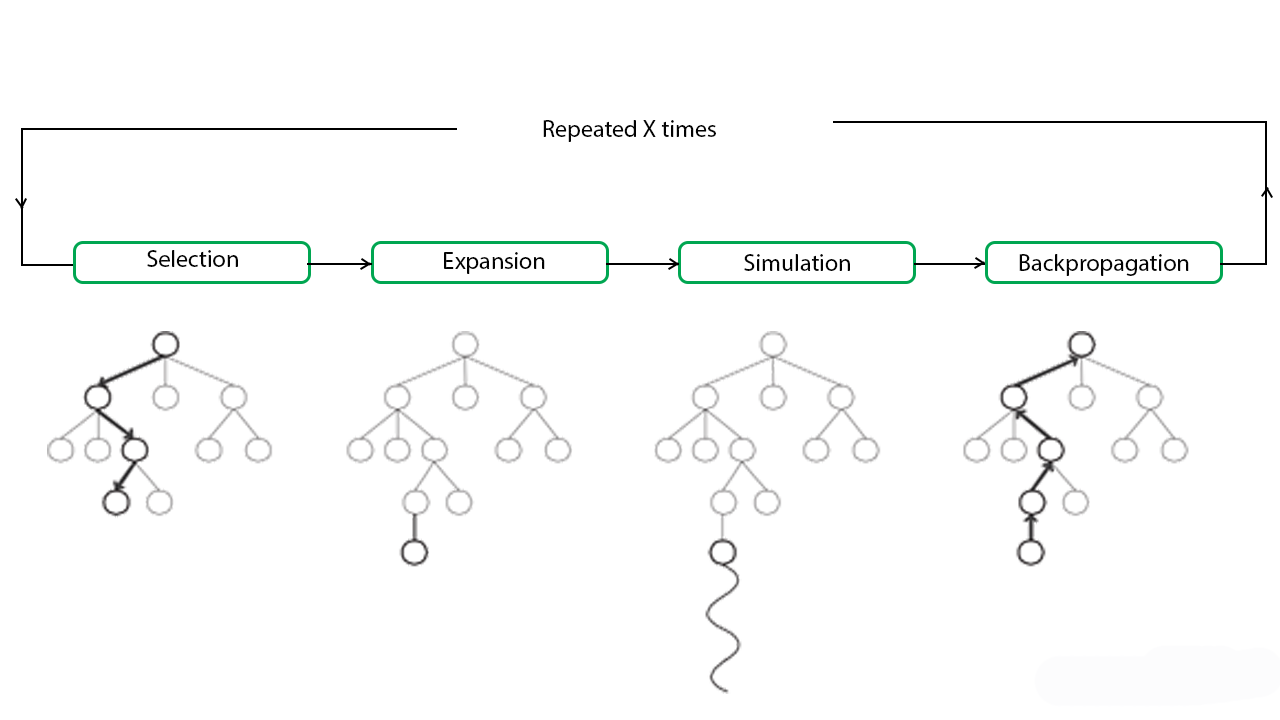
\includegraphics[width=0.9\textwidth]{obrazky-figures/mcts}
	\caption{Diagram jednotlivých fází MCTS.\@
  Zdroj: \cite{mcts_geeksforgeeks}}\label{fig:mcts}
\end{figure}

Tento algoritmus se skvěle hodí na hry s~nedokonalou či neúplnou informací, jelikož se spoléhá na vzorkování pomocí simulací.

\section{Q-learning}\label{subsec:q-learning}

Q-learning je jedním z~nejznámějších algoritmů posilovaného učení.
Učení tohoto algoritmu probíhá bez modelu a mimo strategii.

Jak už název vypovídá, Q-learning se zaměřuje na určení hodnoty hodnotové funkce akce $Q(s, a)$, viz. \ref{subsubsec:q_function}.
Tyto hodnoty se uchovávají v~Q--tabulce, která na každou kombinaci stavu a akce uchovává hodnotu $Q(s, a)$.
Hodnoty v~Q--tabulce se iterativně aktualizují na základě získaných odměn.
Kladná odměna po vykonání akce $s$, zvýší se hodnota $Q(s, a)$.
Naopak, dostane--li po vykonání této akce zápornou odměnu, hodnota $Q(s, a)$ se sníží.

Řádky Q-tabulky tedy reprezentují stavy a sloupce akce.
Po vytvoření jsou všechny $Q$ hodnoty v~tabulce inicializovány na nulu.
Následně jsou tyto hodnoty iterativně aktualizovány dle zpětné vazby udělené od prostředí ve formě odměny.

Jako u~většiny algoritmů je zde potřeba dohlédnout na rovnováhu mezi explorací a exploatací.
K~tomuto se využívá $\epsilon$--greedy strategie viz. \ref{epsilon_greedy}.

Hlavní nevýhodou tohoto algoritmu je právě jeho závislost na Q--tabulce.
Tabulka mapuje hodnoty pro každou kombinaci stavu a akce,
Je--li avšak stavový, či akční prostor příliš velký, nebo dokonce nekonečný je tento algoritmus nevhodný, skoro až nepoužitelný.
Výsledná Q--tabulka by byla neefektivní kvůli své velikosti.
Mohlo by se stát, že s~nekonečným množstvím kombinací by velikost tabulky rostla do \uv{nekonečna}.
Jako řešení byl navrhnut algoritmus Deep Q-learning.

\section{Deep Q-learning (DQN)}\label{subsec:deep-q-learning}

Tato metoda je rozšířením algoritmu Q-learning které,
nahrazuje $Q$--tabulku neuronovou sítí určené k~aproximaci hodnotové funkce akce $Q(s, a)$.
Díky této aproximaci je možné použít tento algoritmus na problémy s~velkým, či nekonečným množstvím kombinací akcí a stavů.

Avšak tímto vzniká nový problém, \emph{nestabilita učení}.
Ten je řešen dvěma mechanizmy:

\begin{itemize}
  \item \textbf{Přehrání zkušenosti (experience replay)}
  
  Během trénování se ukládají všechny zkušenosti do paměti.
  Ať už to jsou akce, stavy, odměny atd.
  Při trénování se poté náhodně vybírají náhodně zkušenosti z~této paměti a aktualizují se podle nich váhy sítě.
  Tímto se snižuje rozdíl mezi jednotlivými aktualizacemi a tím pádem se zvyšuje stabilita učení.
  

  \item \textbf{Periodická aktualizace}
  Síť je naklonována a změny se provádí pouze na duplikátní verzi.
  Do hlavní originální sítě se změny klonují po určitém počtu kroků.

\end{itemize}

Při vytvoření neuronové sítě jsou váhy inicializovány náhodně.

\section{Gradient strategie}\label{subsec:gradient-strategie}
Oproti předchozím zmiňovaným algoritmům, které usilují o~naučení hodnotové funkce či prohledávají stavový prostor, algoritmy gradientu strategie se snaží naučit strategii přímo.

V~diskrétním prostoru je odměnová funkce definována jako:
\begin{equation}
  \label{eq:odmenova_funkce}
  \mathcal{J}(\theta) = V_{\pi_\theta}(S_1) = \mathbb{E}_{\pi_\theta}[V_1]
\end{equation}

Ve~spojitém prostoru je odměnová funkce definována jako:
\begin{equation}
    \label{eq:odmenova_funkce_spojita}
  \mathcal{J}(\theta) = \sum_{s \in \mathcal{S}} d_{\pi_\theta}(s) V_{\pi_\theta}(s) = \sum_{s \in \mathcal{S}} \Big( d_{\pi_\theta}(s) \sum_{a \in \mathcal{A}} \pi(a \vert s, \theta) Q_\pi(s, a) \Big)
  \end{equation}

\begin{itemize}
  \item $\mathcal{J}(\theta)$ je odměnová funkce strategie $\pi_\theta$.
  \item $\theta$ je parametr strategie $\pi_\theta$.
  \item $V_{\pi_\theta}(S_1)$ je hodnota stavu $S_1$ dle strategie $\pi_\theta$.
  \item $\mathbb{E}_{\pi_\theta}[V_1]$ je očekávaná hodnota stavu $S_1$ dle strategie $\pi_\theta$.
  \item $d_{\pi_\theta}(s)$ je rozdělení pravděpodobnosti stavů $s$ dle strategie $\pi_\theta$.
\end{itemize}

\subsubsection*{Věta o~gradientu strategie}
Výpočet gradientu matematicky je zaznamenán touto rovnicí:

\begin{equation}
  \label{eq:gradient_strategie}
  \frac{\partial \mathcal{J}(\theta)}{\partial \theta_k} \approx \frac{\mathcal{J}(\theta + \epsilon u_k) - \mathcal{J}(\theta)}{\epsilon}
\end{equation}
Tento výpočet je velmi pomalý a náročný na výpočet.
Avšak tento vzorec lze zjednodušit na rovnici zvanou \emph{věta o~gradientu strategie}:

\begin{equation}
    \label{eq:veta_o_gradientu_strategie}
  \nabla \mathcal{J}(\theta) = \mathbb{E}_{\pi_\theta} [\nabla \ln \pi(a \vert s, \theta) Q_\pi(s, a)]
\end{equation}


\section{Trust Region Policy Optimization (TRPO)}\label{sec:trust-region-policy-optimization}
Trénované strategie jsou často velmi náchylné na změny.
Kde i malá náhlá změna v~jednom kroku může způsobit velké změny v~chování agenta a zamezit dalšímu učení správné strategie.
Během učení totiž chceme, aby učení probíhalo plynule a ne skokově.
Pokud se strategie změní příliš rychle protože následovala nejstrmější směr růstu, může se stát, že mine cestu vedoucí k~optimální strategii.
Může tedy uváznout v~lokálním optimu.

TRPO je optimalizační algoritmus, který se snaží tento problém řešit tím, že definuje omezení rozdílu mezi novou aktualizovanou strategií $\textbf{p}$ a starou strategií z~předešlého kroku $\textbf{q}$.
Tento rozdíl mezi dvěma pravděpodobnostními rozděleními je definován jako Kullback-Leiblerova divergence (K-L divergence)\cite{KL_divergence}.
Vzorec pro K-L divergenci ve spojitém prostoru je následující:
\begin{equation}
  D_{KL}(p \| q) = \int_x p(x) \log \frac{p(x)}{q(x)} dx
\end{equation}

Vzorec v~diskrétním prostoru:
\begin{equation}
  D_{KL}(p \| q) = \sum_x p(x) \log \frac{p(x)}{q(x)}
\end{equation}

Vzniká tak region důvěry, ve kterém musí nová strategie setrvat.
Strategie se tedy nemůže skokově změnit na lokální maximum, ale pouze následuje směr lokálního maxima.

K~tomu využívá Hessovy matice.
Kdy pomocí těchto matic hledá optimální směr změny strategie.
Tím, že se hledá lokální maximum pouze v~oblasti důvěry, řeší problém se zaseknutím v~těchto lokálních optimech.
Hessova matice je vždy čtvercového tvaru.
Její hodnoty obsahují druhé parciální derivace funkce a popisuje tím její lokální zakřivení.
Jelikož je strategie pravděpodobnostní funkce, jsou tyto matice ideální pro hledání optimálního směru změny strategie.

Díky tomuto řešení se učení stává robustním a stabilním.
Avšak výměnou za to, je náročnost aproximace pomocí Hessových matic a s~tím související náročnost na implementaci.
Výpočet buňky v~Hessovy matici je definován jako:
\begin{equation}
  H_{ij} = \frac{\partial^2 f}{\partial x_i \partial x_j}
\end{equation}
Kde $i$ značí řádek a $j$ sloupec matice.
Výsledná matice tak poté může vypadat takto:

\begin{equation}
  \begin{bmatrix}
     \frac{\partial^2 f}{\partial x_1^2} & \frac{\partial^2 f}{\partial x_1 \partial x_2} \\
     \frac{\partial^2 f}{\partial x_2 \partial x_1} & \frac{\partial^2 f}{\partial x_2^2}
   \end{bmatrix}
\end{equation}

\section{optimalizace proximální strategie (PPO)}
\label{sec:proximalni-optimalizace-strategie}

%\textsuperscript {\ref{sec:trust-region-policy-optimization}}

Metoda optimalizace proximální strategie (Proximal policy optimization - PPO) byla představena roku 2017 \cite{PPO_paper}.
Tato metoda je vylepšeným následníkem algoritmu TRPO, popsaný v~předchozí sekci~\ref{sec:trust-region-policy-optimization}.

Co výrazné odlišuje tuto metodu od předchůdců, je její jednoduchost a efektivita.
Dosahuje lepších výsledků než metoda TRPO a srovnatelných výsledků s~metodou ACER\@.
Je avšak mnohem jednodušší na implementaci, má nižší nároky na výkon a je mnohem lepší co se týče efektivity dat pro trénování \cite{PPO_paper}.
K~dosažení těchto výsledků, využívá PPO techniku ořezávání náhradních cílů vloženou do algoritmu TRPO\@.
Vynucuje, aby K-L divergence staré a nové strategie byla v~rozmezí $[1-\epsilon, 1+\epsilon]$ kde $\epsilon$ je modifikovatelný parametr.

Nechť $r_t(\theta)$ je pravděpodobnostní poměr mezi novou a starou strategií.
\begin{equation}
  r_t(\theta) = \frac{\pi_\theta(a_t \vert s_t)}{\pi_{\theta_{old}}(a_t \vert s_t)}
\end{equation}

Pokud tento vzorec dosadíme do rovnice pro výpočet gradientu strategie TRPO. Kde TRPO využívá K-L divergenci a maximalizuje vedlejší cíle \cite{policy_gradients}, vznikne následovná rovnice:

\begin{equation}
  L^{CLIP}(\theta) = \mathbb{E}_t \Big[ \min \Big( r_t(\theta) \hat{A}_t, \text{clip}(r_t(\theta), 1-\epsilon, 1+\epsilon) \hat{A}_t \Big) \Big]
\end{equation}

\begin{equation}
  L^{CLIP}(\theta) = \mathbb{E}_t \Big[ \min \Big( r_t(\theta) \hat{A}_t, \text{clip}(r_t(\theta), 1-\epsilon, 1+\epsilon) \hat{A}_t \Big) \Big]
\end{equation}

\begin{itemize}
  \item $\theta$ je parametr strategie.
  \item $\mathbb{E}_t$ značí empirickou očekávání v~časových krocích
  \item $r_t$ relativní podobnost nové a staré strategie \cite{PPO_paper}
  \item $\hat{A}_t$ je odhad výhody akce v~čase $t$.
  \item $\epsilon$ je hyperparametr, obvykle nastaven na hodnotu $0.1$ nebo $0.2$.
\end{itemize}

\begin{figure}[H]
	\centering
	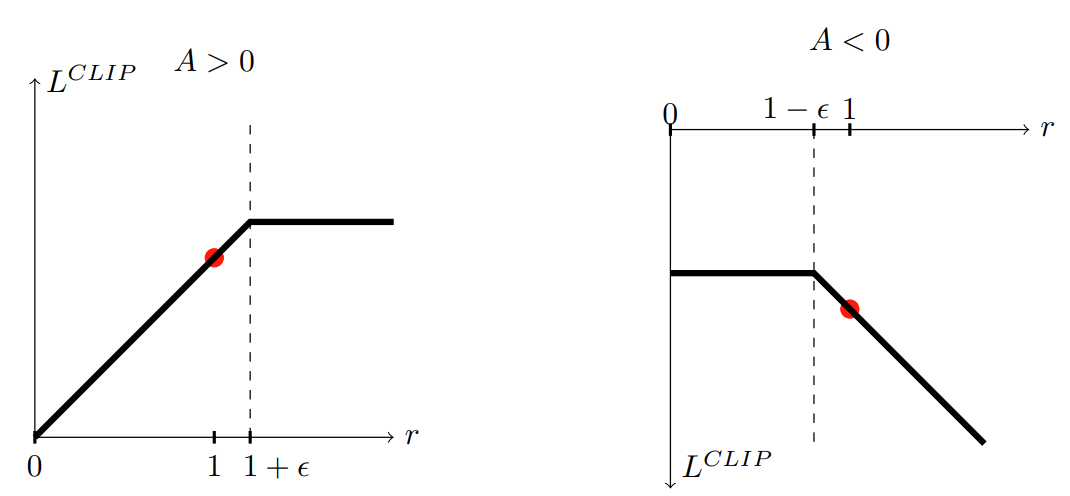
\includegraphics[width=0.6\textwidth]{obrazky-figures/clip}
	\caption{Grafy zobrazují 1 časový krok funkce $L^{CLIP}$. Červeným bodem je označen počáteční stav optimalizace. Levý graf zobrazuje kladnou změnu a pravý zápornou změnu.
  Zdroj: \cite{RL_basics}}\label{fig:clip}
\end{figure}

Tyto změny tvoří PPO oproti TRPO kompatibilní s~metodou stochastického gradientního sestupu.
Odstraňuje K--L omezení a nahrazuje je ořezáváním.

PPO má však i své nedostatky.
\label{PPO_weakness}
Dle studie~\cite{PPO_weakness} se ukázalo, že PPO nefunguje optimálně za 3 podmínek:
\begin{enumerate}
  \item V~prostředí se spojitým prostorem akcí je nemodifikované PPO nestabilní, pokud odměna náhle zmizí mimo ohraničenou podporu.
  \item V~diskrétním akčním prostoru s~řídkými a vysokými odměnami PPO volí neoptimální akce.
  \item V~době těsně po inicializaci je náchylné k~předčasné volení strategie, pokud je některá z~optimálních akcí po inicializaci blízko a snadno dosažitelná.
\end{enumerate}

Tato studie také navrhla tyto řešení a prokázala jejich účinnost.
Bod 1 a 3 je řešen buď převedením spojitého akčního prostoru na diskrétní nebo zavedením \emph{Beta parametrizace strategie}.
\emph{KL regulováním cíle} je řešen bod 2.

Podmínka číslo 1 je v~mé implementaci prostředí hry Scotland Yard implicitně neplatná, jelikož akční prostor je diskrétní.\\
Podmínka číslo 2 je řešena přidáním menších dílčích odměn.
Agenti tak získávají odměny i za menší kroky, nejen například za vítězství/ prohru či blízkost, viz. podsekce~\nameref{subsubsec:odmeny}.\\

\begin{algorithm}
  \caption{Proximal Policy Optimization (PPO)}
  \begin{algorithmic}[1]
  \Require Počáteční parametry politiky $\theta_0$, počáteční parametry hodnotové funkce $\phi_0$
  \For{iterace $= 0, 1, 2, \dots$}
      \State Shromáždí sadu trajektorií $\mathcal{D}$ spuštěním politiky $\pi_\theta$ v prostředí
      \State Vypočítej odměny trajektorií $\hat{R}_t$
      \State Vypočítej odhady výhod $\hat{A}_t$ pomocí aktuální hodnotové funkce $V_{\phi_k}$:
      \[
      \hat{A}_t = \sum_{t'=t}^T \gamma^{t'-t} r_{t'} - V_{\phi_k}(s_t)
      \]
      \State Aktualizuj parametry politiky $\theta$:
      \[
        \theta_{k+1} = argmax_{\theta} \frac{1}{\left|\mathcal{D}_k\right|T}\displaystyle\sum_{\tau \in \mathcal{D}_k} \sum_{t=0}^T \left[ \min \left( r_t(\theta) \hat{A}_t, \text{clip}(r_t(\theta), 1-\epsilon, 1+\epsilon) \hat{A}_t \right) \right]
      \]
    \EndFor
  \end{algorithmic}
  \end{algorithm}\pagebreak
  \begin{itemize}
    \item $k$ - iterace
    \item $r_t(\theta) = \frac{\pi_\theta(a_t|s_t)}{\pi_{\theta_{old}}(a_t|s_t)}$\\ - poměr šance zvolení akce $a_t$ ve stavu $s_t$ \\ mezi novou a předchozí politikou
    \item $\epsilon$ - hyperparametr klipoavací funkce.
    \item $\text{clip}(r_t(\theta), 1-\epsilon, 1+\epsilon) \hat{A}_t$ - klipovaná ztráta politiky
    \item $r_t(\theta) \hat{A}_t$ - ztráta politiky
    \item min -  vybere nejmenší změny aby nedošlo k nestabilitě učení.
    \item $\hat{A}_t$ - odhadovaná výhoda akce $a_t$ ve stavu $s_t$
    \item $\frac{1}{\left|\mathcal{D}_k\right|T}$ - počet trajektorií v sadě $\mathcal{D}_k$ a počet kroků $T$ v trajektorii
    \item $\displaystyle\sum_{\tau \in \mathcal{D}_k} \sum_{t=0}^T$ - sumace přes všechny trajektorie v sadě $\mathcal{D}_k$ a všechny kroky $t$ v trajektorii
    \item $argmax$ - hledá takový argument, který maximalizuje funkci. Pomocí optimalizačních metod (Adam, nebo gradientní sestup)
\end{itemize}



\chapter{Implementace systému pro autonomní hraní hry Scotland Yard}
\label{ch:navrh}
V~této kapitole je popsáno navržené řešení a výsledná implementace.
\section{Zkoumaná modifikovaná verze hry Scotland Yard}\label{sec:zkoumana-modifikovana-verze-hry-scotland-yard}

Tato práce využívá modifikovanou verzi hry Scotland Yard, ve které se hráči pohybují po mřížkové herní ploše ve tvaru čtverce.
Na mřížce se nachází 15$\times$15 polí.
Hráčí se po těchto polích mohou pohybovat ortogonálně i diagonálně, vždy však o maximálně 1 pole.
Hráč se může rozhodnout nezměnit pozici a zůstat na svém aktuálním poli.
K~pohybu nejsou potřebné žádné jízdenky.

Předtím nežli začne hra, se vyberou náhodné možné pozice na kterých mohou Pan~X a policisté začínat.
Z~těchto možných pozic se následně náhodná pozice přidělí jednotlivým hráčům.
Poté začíná hra.

Hra se dělí na jednotlivá kola, ve kterých se hráči ve svých tazích střídají.
Pro hru byli zvoleni 3 policisté, z~toho důvodu, že je herní pole velké a 2 policisté by nemuseli mít možnost ho celé pokrýt.
V~kole hraje jako první Pan~X a poté policisté, již podle jejich očíslování, které jim bylo náhodně přiděleno při vytvoření.
Hra končí v~okamžiku, kdy policisté chytí Pana~X nebo když Pan~X zůstane nepolapen až do konce.

Z~původní verze hry byly odstraněny některé elementy jako jsou jízdenky a různé druhy dopravních prostředků.
Tato úprava vede k~tomu, že se zjednodušil stavový i akční prostor, jelikož se nemusí starat o~svoje jízdenky a mohou se pohybovat po herní ploše libovolně.
Změny, avšak nemění základní podstatu hry, zachovává neurčitost, ale značně zjednodušuje implementaci.
Díky tomuto zjednodušení klade trénování nižší nároky na výkon.

\section{Implementace uživatelského rozhraní a herních mechanizmů}\label{subsec:implementace-uzivatelskeho-rozrani-a-hernich-mechanizmu}

Uživatelské rozhraní bylo vytvořeno pomocí knihovny \texttt{Pygame}.
Hra začíná v~menu, kde je momentálně možné vybrat pouze možnost sledování hry mezi dvěma agenty.
Je zde ale možnost vybrat jaký algoritmus rozhodování je použit pro jednotlivé agenty.
K~dispozici jsou algoritmy \emph{PPO}, \emph{DQN} a náhodné chování.

\begin{figure}[H]
	\centering
	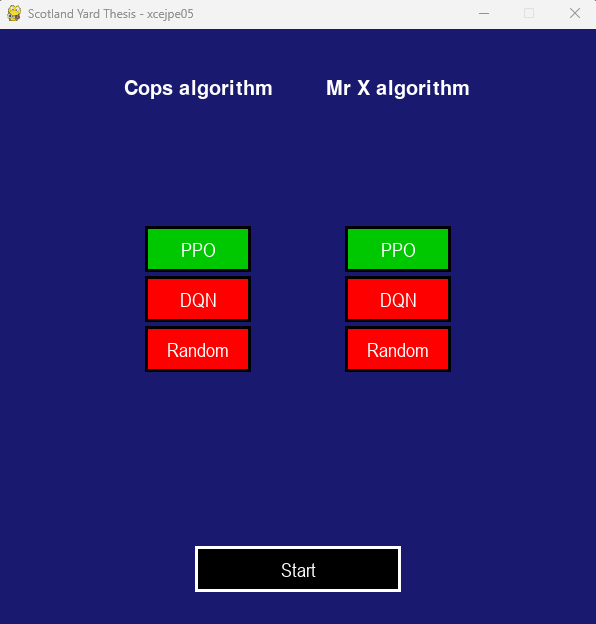
\includegraphics[width=0.7\textwidth]{obrazky-figures/game_title}
	\caption{Menu hry}\label{fig:game_title}
\end{figure}

Samotný kód hry je rozdělen na 3 částí.
Jednotlivé vrstvy hry jsou tak izolovány a mohou být snadno vyměněny za jiné implementace.

\begin{itemize}
  \item \emph{GameController}~\cite{GameSceneController}
  
  Tato třída je zodpovědná za řízení hry.
  Je zde spuštěna univerzální herní smyčka, která zpracovává uživatelské vstupy.
  A~následně provádí aktualizaci stavu aktuální scény a překreslení dané scény.
  \item \emph{Scény}~\cite{GameSceneController}
  
  Jednotlivé scény následně definují své chování při aktualizaci a překreslení.
  Manipulace a přepínání mezi nimi je zajištěno pomocí zásobníků scén.
  Do tohoto zásobníku se ukládají nově otevřené scény a obsluhována je vždy ta nejnovější.

  \item \emph{Hra}

    Samotná hra je následovně rozdělena na 2 další části která každá zpracovává jinou část hry.\vspace{-0.5em}
    \begin{itemize}
      \item \emph{Herní logika} --- src/game/scotland\_yard\_game\_logic.py
      Zpracovává herní mechanizmy, jako je pohyb, zpracování výherních podmínek atd.
      Zprostředkovává informace pro prostředí a to poté pro učící se agenty.

      \item \emph{Herní vizualizace} ---  src/game/scotland\_yard\_game\_visual.py
      Vykreslování herních elementů (herní pole, figury atd.).
    \end{itemize}
\end{itemize}

\textit{Použití herní smyčky, která obsluhuje aktuální scénu bylo inspirován výukovým projektem z~platformy GitHub~\cite{GameSceneController}.
Kód byl, avšak značně upraven a vylepšen, aby vyhovoval integrování do této práce.}

Hra se zapne v~pozastaveném stavu, aby bylo možné lépe pozorovat počáteční rozložení hráčů.
Pokud je hra pozastavena, je možné pokračovat stisknutím klávesy Space (mezerník).
Jakmile hra běží, je možné ji opětovně pozastavit stisknutím klávesy Space (mezerník).


Na herní ploše jsou zobrazeny 4 figury ve formě barevného čtverce.
Červený čtverec značí Pana~X a zelené čtverce značí policisty.
V~levém horním rohu okna je zobrazen aktuální stav hry.
Pakliže hra stále běží, je zobrazeno číslo aktuálního kola.
Jakmile hra skončí, je zobrazeno, kdo hru vyhrál.
Za 

\begin{figure}[H]
	\centering
	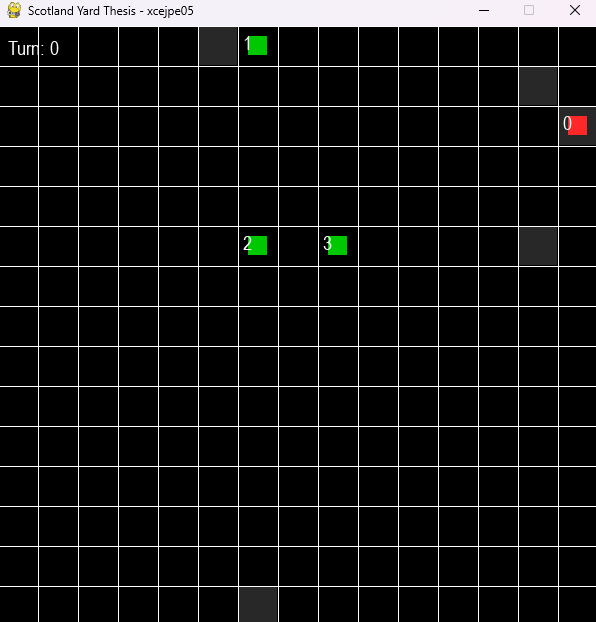
\includegraphics[width=0.8\textwidth]{obrazky-figures/game_0}
    \caption{Hra před spuštěním}
    \label{fig:game_0}
\end{figure}

V~obrázku~\ref{fig:game_0} je hra v~pozastaveném stavu a je zobrazeno počáteční rozložení hráčů.
Na obrázku lze vidět tmavě šedé čtverce, které značí možnou pozici Pana~X\@.
Na začátku hry, je těchto pozic mnoho, jelikož Pan~X doposud svoji pozici neodhalil.

\begin{figure}[H]
	\centering
	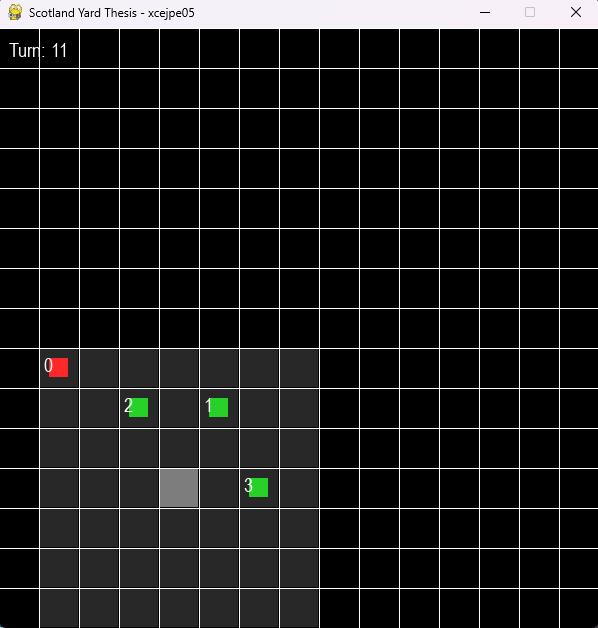
\includegraphics[width=0.8\textwidth]{obrazky-figures/game_11}
      \caption{Jedenácté kolo hry}
    \label{fig:game_11}
\end{figure}

Na obrázku~\ref{fig:game_11} je zobrazeno jedenácté kolo hry.
Světlé šedý a nejvýraznější čtverec značí poslední známou pozici Pana~X\@.
Tmavě šedé čtverce opět značí možné pozice Pana~X\@.
Na tomto obrázku lze pozorovat, že policisté jsou v~blízkosti Pana~X a snaží se ho chytit.
Všichni policisté se z~pozic, zobrazených na obrázku~\ref{fig:game_0}, přesunuli na možné pozice Pana~X\@.

\section{Prostředí a učení agentů}
\label{sec:implementace}

\subsection{Použitá knihova pro učení}\label{subsec:pouzite-technologie}
K~učení modelů pro hru Scotland Yard byl využit open-source framework \texttt{Ray}~\cite{Ray}.
Konkrétně byla využita knihovna \texttt{Ray.Rllib}.
Tato knihovna poskytuje nástroje pro posilované učení a samotné implementace jednotlivých algoritmů, včetně zkoumaného algoritmu \emph{PPO}.
Rllib dokáže využívat obě populární knihovny pro strojové učení \texttt{Tensorflow} a \texttt{Pytorch}.
Pro tuto práci byla vybrána knihovna \texttt{Pytorch}.

Knihovna \texttt{Ray} byla zvolena pro podporu učení více modelů naráz, je vhodná pro velké projekty a umožňuje možnosti konfigurace jako žádný jiný framework.
Obsahuje spoustu implementací algoritmů pro posilované učení a jelikož je má výsledná implementace modulární, lze jednoduše zaměnit využívaný algoritmus za jiný.

Prvotní konfigurace a vytvoření prostředí je ale složité, jelikož dokumentace pro konfiguraci jednotlivých algoritmů není příliš komplexní.

\subsection{Pozorovací a akční prostor agentů}
V~této práci vzájemně v~prostředí vystupují dva agenti s~různými strategiemi a různými pozorovacími prostory.
Akční prostor je stejný jak pro policisty, tak pro Pana~X\@.
Oba prostory jsou diskrétní

\bigskip
\textbf{Pozorovací prostor} agentů je velmi důležitý pro úspěšné naučení dobré strategie.
Struktura jednotlivých pozorovacích prostorů je následující:

\begin{itemize}
  \item Shodné položky
    \begin{itemize}
    \item Pozice X, Y sama sebe
    \item Pozice X, Y a vzdálenost od poslední známé pozice pana~X
    \item Číslo aktuálního kola
    \item Maximální počet kol
    \item Číslo kola, kdy dojde k~dalšímu odhalení pozice Pana~X
  \end{itemize}
  \item \textbf{Pan~X}
    \begin{itemize}
    \item Pozice X, Y policistů
    \item Vzdálenost od  policistů
  \end{itemize}
  \item \textbf{Policisté}
    \begin{itemize}
    \item Pozice X, Y zbylých policistů
    \item Vzdálenost od zbylých policistů
    \item Pozice X, Y nejbližšího bodu oblasti zájmu
    \item Vzdálenost od nejbližšího bodu oblasti zájmu
    \item Pravdivostní hodnota, zda je policista v~oblasti zájmu
  \end{itemize}
\end{itemize}

Agenti tedy nevidí všechny pole, ale jen ty které jsou důležité.
Důležitý je observační prostor policistů.
Ti vidí pouze poslední známou pozici Pana~X a oblast zájmu.
Oblast zájmu je oblast ve které se může Pan~X nacházet.
Je to obdoba reálného hledání, kde také známe rychlost sledovaného objektu a jeho poslední známou pozici.

Přidání této oblasti bylo esenciální, protože bez ní by policisté dostávali jen velké a velmi řídké odměny pouze pokud by chytili Pana~X\@.
Takto je zajištěno, že dostávají i menší, dílčí odměny za to, že se pohybují v oblasti kde se Pan X nachází\@.

\begin{figure}[H]
	\centering
	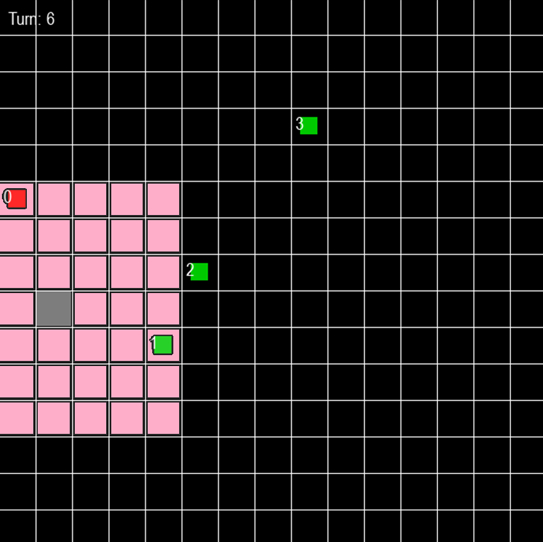
\includegraphics[width=0.6\textwidth]{obrazky-figures/interest_area}
      \caption{Zvýrazněná oblast zájmu policistů (růžové pole).}
    \label{fig:game_11}
\end{figure}

Pokud informace obsažená v~těchto pozorovacích prostorech není v~daný moment definována, je nahrazena hodnotou -1.
Konkrétně se jedná pouze o~hodnoty týkající se poslední veřejně známé pozice Pana~X, jelikož v~prvních několika kolech není známa.

\bigskip

\textbf{Akční prostor} agentů reprezentuje možné akce, které mohou agenti provést.
Tyto akce jsou stejné jak pro policisty, tak pro Pana~X\@.
Agenti se mohou hýbat ortogonálně i diagonálně.
Ale také můžou zůstat na místě.
Celkově tedy agent může zvolit z 9 akcí.

\subsection{Trénování agentů pomocí algoritmu DQN a PPO}

Agenti se již od začátku učí zásadně pouze hraním proti sobě.
Důvodem pro toto rozhodnutí bylo, že se jedná o~zajímavější experiment, kdy jsou agenti vpuštěni do zcela neznámého prostředí a nemají se od koho učit strategii.
Jejich učení tedy není nijak podporováno a musí se naučit strategii sami.
Tím je i pozorováno, jestli jsou agenti vůbec schopni rozpoznat cíl hry, co je po nich požadováno a případně jak rychle dosáhnou dobré strategie.

Trénování modelů je ve dvou skriptech:
\begin{itemize}
  \item TrainerDQN.py
  \item Spuštení: \texttt{python TrainerDQN.py {\color{red}DOPSAT FLAGY}}
  \begin{itemize}
    \item --do-backup: během ukládání vytvoří záložní kopii modelu
    \item --backup-folder [string]: složka pro záložní kopie; default: none
    \item --load-folder [string]: načte model z~dané složky; default: trained\_model\_dqn
    \item --save-folder [string]: uloží model do dané složky; default: trained\_model\_dqn
    \item --num-iterations [int]: počet iterací trénování; default: 50
    \item --save-interval [int]: interval ukládání modelu
    \item --verbose
  \end{itemize}
  \item TrainerPPO.py
\end{itemize}

Tyto spustitelné skripty obsahují konfigurace pro trénování modelů.
Při spuštění skriptu se načte aktuální model, pokud existuje a pokračuje v~trénování tohoto modelu.
Pokud model neexistuje, je vytvořen nový model a začíná se s~trénováním od začátku.
Model je uložen každých 5 iterací trénování.
Při dlouhém trénování doporučuji spustit script s parametrem \texttt{--do-backup}, který zároveň vytvoří záložní kopii modelu.
Během několikadenního trénování může dojít k výpadku proudu, či jiné chybě a model může být poškozen.

\subsubsection*{Neuronové sítě ve výsledných modelech}
V modelech PPO i DQN hraje hlavní roli neuronová síť.
Vstupem do těchto neuronových sítí je aktuální stav, v tomto případě viditelné pozorování z prostředí, popsané v předchozí části.
Tyto vstupy jsou následně zpracovány skrytými vrstvami v jednotlivých neuronových sítích.
Struktura vnitřních vrstev a výstup neuronové sítě jsou rozdílné pro oba algoritmy.
\bigskip

  \textbf{Neuronová síť v PPO}
    \begin{itemize}
      \item Vstup
        \begin{itemize}
          \item viditelný stav prostředí
        \end{itemize}
      \item Struktura
        \begin{itemize}
          \item vstupní vrstva má 17 vstupů pro Pana~X a 18 pro policisty
          \item dvě skryté vrstvy po 256 neuronech [256, 256]
          \item 9 výstupů (1 pro každou akci)
        \end{itemize}
      \item Výstup
        \begin{itemize}
          \item Výstupem této neuronové sítě je pravděpodobnostní rozdělení nad všemi akcemi.
          \item Jedná se tedy o stochaistickou strategii, kde každá akce má šanci na zvolení, některá větší a některá menší, kde tuto šanci určuje neuronová síť.
        \end{itemize}
    \end{itemize}

    \textbf{Neuronová síť v DQN}
    \begin{itemize}
      \item Vstup
        \begin{itemize}
          \item viditelný stav prostředí
        \end{itemize}
      \item Struktura
        \begin{itemize}
          \item vstupní vrstva má 17 vstupů pro Pana~X a 18 pro policisty
          \item dvě skryté vrstvy, kde první má 128 neuronů a druhá 64 [128, 64]
          \item 9 neuronů výstupní vrstvy
        \end{itemize}
      \item Výstup
        \begin{itemize}
          \item Výstupem této neuronové sítě je ohodnocení všech akcí (Q hodnota akce).\\
          \item Používám $\epsilon-greedy$ variantu.
          Následně se tedy tyto hodnoty porovnají a vybere se akce s největší Q hodnotou.
        \end{itemize}
    \end{itemize}


  \bigskip

  Agenti během učení modifikují vahy neuronů ve skrytých vrstvách svého modelu pro dosáhnutí požadovaného chování.
  Ve výsledné aplikaci již agenti obdrží od prostředí pozorování, které dají na vstup neuronové sítě svého modelu a na základě výsledků zvolí akci.

Implementace algoritmu PPO i DQN je obsažena v~knihovně \texttt{Ray.Rlib}.
PPO využívá základní parametry trénování bez žádné modifikace parametrů jelikož se ukázalo, že agenti se chovají optimálně a hru pochopili i bez těchto zásahů do výchozích hodnot hyperparametrů.
Zato DQN agenti se chovali \emph{ne}optimálně.
Agenti se naučili pouze stát na místě, přestože tato taktika byla velmi nevýhodná.
Pro vyřešení tohoto problému, je nyní agentům udělována penalizace pokud se 5 kroků po sobě nepohnou.
Penalizace je rovna zápornému počtu kol nečinnosti.
Postupně tedy roste a pohybem je resetována.
Tato expanze odměn vedla k~vylepšení strategie agentů DQN a nadále nestáli pouze na jednom místě.
Bohužel však přes veškeré snahy, agenti DQN nedosahují ani zdaleka tak dobrých výsledků jako agenti PPO\@.

S~konfiguračními parametry \texttt{Ray.rlib}u a hyperparametry DQN jsem dlouho experimentoval.
Měnila se velikost vnitřních vrstev, počet neuronů, rychlost učení, velikost paměti, velikost dávky učení a další.

Výsledná konfigurace je následující.
Obsahuje 2 vnitřní skryté vrstvy, první vrstva má 128 neuronů a druhá vrstva má 64 neuronů.
Používá verzi \emph{double DQN}
Algoritmus k~vyvážení explorace a exploatace při učení využívá metodu $\epsilon$--greedy, kde je $epsilon$ postupem trénování lineárně snižováno z~hodnoty 1 na 0.05.
Tato hodnota udává pravděpodobnost náhodné volby akce.
Po natrénování modelu je ve hře explorace vypnuta, $epsilon$ je tedy nastaveno na 0.
K~posílení explorace během trénování je k~vahám sítě přidán \uv{šum}.
Pro zlepšení stability je povoleno přehrávání zkušeností.
Avšak i přesto jsou výsledky agentů DQN neuspokojivé, viz.\nameref{ch:experimenty}.

\subsubsection*{Řešení zvolení nevalidních akcí}

Hra Scotland Yard má omezené herní pole.
Tím pádem je jasné, že pokud se hráči vyskytují na okraji herního pole, nemohou zvolit takovou akci, která by je posunula mimo toto herní pole.
Policisté také nemohou zvolit akci, která by je posunula na stejné pole, ve kterém již je jiný policista.
K~vyřešení tohoto problému se nejčastěji využívá tzv.~ maska akcí (\emph{Action mask}).
Framework Ray tuto možnost v~omezené míře podporuje.
Vytvořené prostředí je, avšak potřeba obalit v~obalové třídě, která tuto funkcionalitu zprostředkuje.
Bohužel se mi nepodařilo tuto funkcionalitu spojit s~dalšími požadavky systému, které také vyžadují zabalení do jiné třídy.
Mezi těmito požadavky je fungování více aktérů s~různými strategiemi v~jednom prostředí a různé pozorovací prostory agentů.

strategie, tedy může zvolit nevalidní akci, ale je za jejich zvolení velmi penalizována.
Agenti ji tedy volí opravdu zřídka, a to jen na základě velmi malé explorační šance a pouze na počátku trénování.
Pokud se i tak stane, je ve hře implementovaná funkcionalita, která se pokusí znovu vygenerovat další akce, dokud vygenerovaná akce není validní.
Aby se zamezilo nekonečnému cyklu čekání na validní akci, je po 100 pokusech vygenerována náhodná validní akce.
Takto uměle generovaná akce, nebyla za celou dobu testování agentů PPO potřeba, avšak ze statistického hlediska může tato situace nastat.

Zavedení tohoto omezení pomocí systému odměn vedlo k~positivním výsledkům a agenti se naučili jaké akce jsou nevalidní a nepoužívají je.

\subsubsection*{Systém odměn}
\label{subsubsec:odmeny}

Jednotlivým agentům jsou udělovány odměny na základě jejich chování.
Jelikož policisté a Pan~X mají odlišné a protichůdné strategie i jejich odměny jsou odlišné.
Odměny které agenti dostávají byly navrženy odhadem a laděny postupným experimentováním.
Konečné odměny jsou vypočítány následovně:

\begin{equation}
    \label{eq:odmena_za_vzdalenost_od_policisty}
  R_{\rho_p} = \rho_{p_c} - \rho_{pref}
\end{equation}
\begin{equation}
    \label{eq:odmena_za_vzdalenost_od_posledni_pozice}
  R_{\rho_l} = \rho_l * 0.2
\end{equation}
\begin{equation}
    \label{eq:celkova_odmena}
  R = R_{\rho_p} + R_{\rho_l}
\end{equation}

\begin{itemize}
  \item $R_{\rho_p}$ - odměna za vzdálenost od policistů
  \item $R_{\rho_l}$ - odměna za vzdálenost Pana~X od jeho poslední známé pozice
  \item $R$ - celková odměna
  \item $\rho_l$ - vzdálenost Pana~X od jeho poslední známé pozice
  \item $\rho_{p_c}$ - vzdálenost nejbližšího policisty od Pana~X
  \item $\rho_{pref}$ - pomezí mezi kladnou a zápornou odměnou.
  Pokud je vzdálenost od policisty menší než tato hodnota, Pan~X obdrží zápornou odměnu a naopak kladnou.
\end{itemize}

Bylo také experimentováno s~variantou kde byla odměna za vzdálenost od policistů počítána pro všechny policisty zvlášť a následně byla zprůměrována:

\begin{equation}
  R_{\rho_p} = \sum_{i=1}^{3}[(\rho_{p_i} - \rho_{pref})] \div 3
\end{equation}

Což ale vedlo k~tomu, že Panu X tolik \uv{nevadilo} když byl blízko jednoho policisty, ale daleko od zbylých dvou.
Výpočet této odměny se tedy změnil na výše uvedený vztah~\ref{eq:odmena_za_vzdalenost_od_policisty}.
Což vedlo ke zlepšení výsledků Pana X.

Výpočet odměny policistů je složitější.
Policisté znají poslední odhalenou pozici Pana~X\@.
Okolo tohoto bodu je vytvořená oblast zájmů, ve které se Pan~X může nacházet.
Policisté znají bod této oblasti, který je jim nejbližší, neboli vstupní bod.
Čím blíže je policista k~tomuto bodu, tím větší odměnu získává.
Pokud je od oblasti velmi vzdálený obdrží penalizaci.
Jakmile policista docílí oblastí zájmů dostává konstantní odměnu za to, že se pohybuje v~lokaci ve které se může objevovat Pan X.

PPO algoritmus může začít v~prostředích s~diskrétními akcemi volit velmi neoptimální akce.
Toto nastává pokud má příliš málo podstatných odměn\cite{PPO_weakness}.
To se dokonce ukázalo i během tohoto experimentu, kdy v~raných fázích vývoje nebyla udělována odměna za vzdálenost od oblasti zájmu.
Učení nebylo příliš úspěšné, ale přidáním této dílčí odměny za interakci s~touto oblastí se výsledná strategie značně zlepšila a agenti dosahovali lepších výsledků.

Tento styl odměňování policistů se ukázal jako velmi efektivní.
Další varianta byla přidat do pozorování policistů pozice všech pozic, kde se může Pan~X nacházet.
Toto by ale bylo méně efektivní, jelikož by se pozorovací prostor několikanásobně zvětšil.
Tím by se zvýšila náročnost výpočtů a zpomalilo by se učení.
\chapter{Experimenty}
\label{ch:experimenty}

Pro ověření vlastností algoritmu PPO byly provedeny dva experimenty.
Experimenty byly prováděny na systému s~následujícími parametry:

\begin{itemize}
  \item Operační systém: Windows 10 (64-bit)
  \item Procesor: Intel Core i5--9300H
  \item Paměť: 16 GB DDR4
  \item Grafická karta: NVIDIA GeForce GTX 1660 Ti
\end{itemize}

Agenti DQN i PPO se učili ve stejném prostředí, za stejných počátečních podmínek, měli totožný stavový i akční prostor a od prostředí získávaly stejné odměny.

Pro uskutečnění těchto experimentů byly vytvořeny skripty v~jazyce Python.
Jeden pro sběr dat a druhý pro jejich následné vyhodnocení a zpracování do grafů a textové podoby.

\section{Experiment 1: Pozorování vývoje chování během tréninku}
\label{sec:experiment-1}

Experiment trénování spočívá v~tom ukázat, jak se agenti postupem trénování zlepšují.
U~agentů DQN a PPO je očekáván nárůst průměrné odměny a snížení průměrné vzdálenosti policistů od Pana~X\@.
Experiment v~průběhu tréninku periodicky provádí simulace her mezi agenty a zaznamenává jejich průběh.

\bigskip
\noindent Hlavními sledovanými parametry jsou:\vspace{-0.5em}
\begin{itemize}
  \item Průměrná odměna Pana~X\vspace{-0.5em}
  \item Průměrná odměna policistů\vspace{-0.5em}
  \item Průměrná vzdálenost policistů od Pana~X\vspace{-0.5em}
  \item Počet vyhraných her Pana~X\vspace{-0.5em}
  \item Počet vyhraných her policistů
\end{itemize}
Experiment sleduje vývoj těchto hodnot po \textbf{1000 iterací}.
Což znamená, že na konci experimentu, podstoupili všichni agenti přesně 1000 iterací tréninku

Simulační hry byly prováděny ve všech možných kombinací algoritmů.
Zkoušeny tedy byly všechny algoritmy jak v~roli Pana~X, tak v~roli policistů.
Simulace byly spouštěny po různém počtu trénovacích iterací v~závislosti na aktuálním počtu již provedených iterací.\pagebreak

Počet simulací byl následovný:\vspace{-0.5em}
\begin{itemize}
  \item 50 simulací každých 10 iterací, do 100 trénovacích iterací\vspace{-0.5em}
  \item 50 simulací každých 20 iterací, od 100 do 500 trénovacích iterací\vspace{-0.5em}
  \item 50 simulací každých 50 iterací, od 500 do 1000 trénovacích iterací
\end{itemize}

Při učení je nejzajímavější sledovat vývoj chování agentů na začátku trénování.
Proto byly simulace prováděny s~větší četností právě na začátku a postupem trénování byla četnost snižována pro snížení výpočetní a časové zátěže simulací.
Tím bylo zajištěno, že experiment správně a efektivně vyobrazuje jak rychle a jestli, agenti byly schopni pochopit cíl hry.
Sběr dat pro tento experiment trval přibližně 18 hodin.
Při četnějším sběru dat by rapidně narostla časová náročnost experimentu a dle testovacích spuštění a výpočtů by trval i několik dní.

\subsection{Výsledky experimentu}
\label{subsec:vysledky-experimentu-1}

Při sledování výsledků tohoto experimentu je důležité si uvědomit že díky základní premise hry Scotland Yard je pro policisty vyhrát mnohem složitější než pro Pana~X\@.
A~to z~toho důvodu, že  policisté dokáží vyhrát pouze pokud chytí Pana~X, zato Pan~X může vyhrát jenom na základě uplynutí maximálního počtu kol.

Všechny následující grafy vyobrazují průměrnou odměnu Pana~X (modrá, nepřerušovaná linie) a policistů (oranžová, přerušovaná linie), průměrnou vzdálenost policistů od Pana~X (zelená, tečkovaná linie) a to vše v~závislosti na počtu trénovacích iterací.

\subsubsection*{Srovnání s~náhodným agentem}
\begin{figure}[H]
  \begin{minipage}{.48\textwidth}
    \centering
    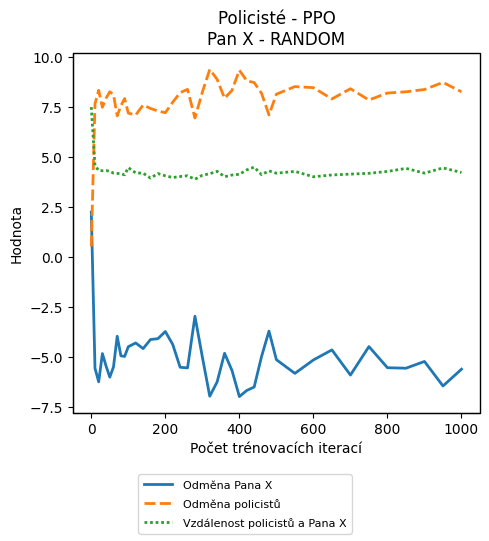
\includegraphics[width=1\textwidth]{obrazky-figures/graphs/cop_PPO_mrx_RANDOM}
    \caption{Graf simulace her mezi policisty trénovanými pomocí PPO a Panem X volícím náhodné akce}
    \label{fig:cop_ppo_mrx_random}
  \end{minipage}\hfill
  \begin{minipage}{.48\textwidth}
    \centering
    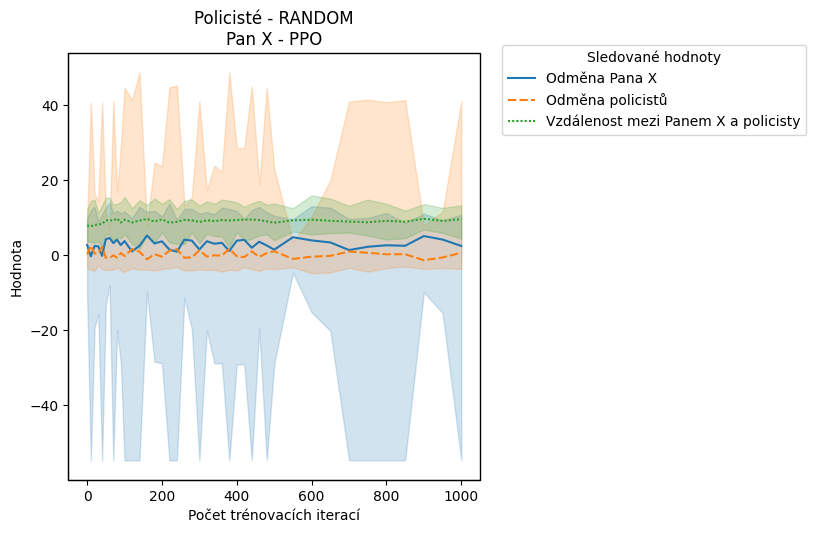
\includegraphics[width=1\textwidth]{obrazky-figures/graphs/cop_RANDOM_mrx_PPO}
      \caption{Graf simulace her mezi Panem X trénovaným pomocí PPO a policisty volícími náhodné akce}
      \label{fig:cop_random_mrx_ppo}
  \end{minipage}
  \end{figure}

Jak jde vidět na grafu~\ref{fig:cop_ppo_mrx_random}, policisté jsou velmi úspěšní ve své strategii.
Vzdálenost mezi policisty, trénovanými pomocí PPO a Panem X, který volí náhodné akce, je po celou dobu velmi malá.
Odměna kterou policisté získávají je velmi vysoká.
Odměna Pana~X je naopak velmi nízká.

Na grafu lze také sledovat že průměrná vzdálenost policistů od Pana~X na začátku trénování rapidně klesá, stejně tak jako klesá odměna Pana~X tím, že se zlepšuje strategie policistů.
Po tomto rapidním poklesu se vzdálenost policistů od Pana~X stabilizuje a odměna Pana~X se drží na nízké hodnotě.

Naopak z~grafu~\ref{fig:cop_random_mrx_ppo} lze pozorovat, že je odměna Pana~X kladná, a až na odchylky vyšší než odměna policistů, kteří se chovají náhodně.
Odměna policistů se pohybuje kolem nuly a odměna Pana~X je stále kladná.
Také vzdálenost policistů od Pana~x je skoro dvojnásobná než v~předchozím případě.

\begin{figure}[H]
  \centering
  \begin{minipage}{.48\textwidth}
    \centering
    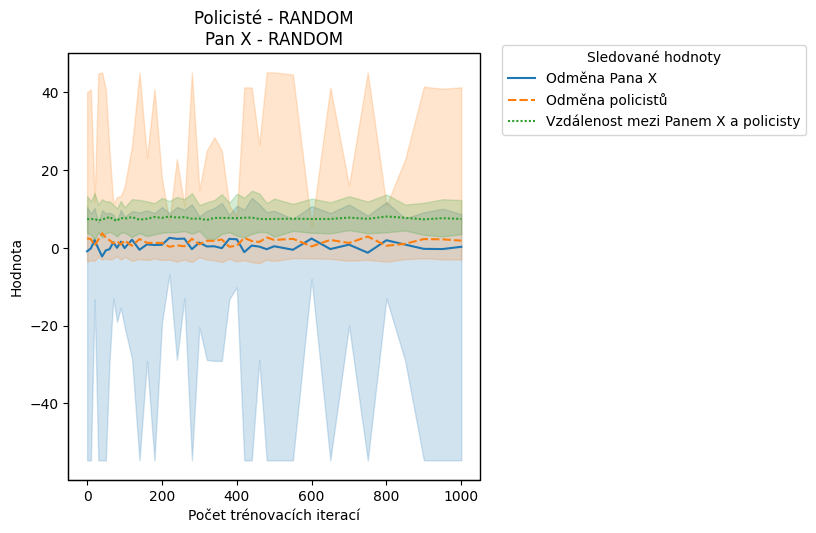
\includegraphics[width=1\textwidth]{obrazky-figures/graphs/cop_RANDOM_mrx_RANDOM}
    \caption{Graf simulace her mezi policisty a Panem X, kde oba volí náhodné akce}
    \label{fig:cop_random_mrx_random}
  \end{minipage}\hfill
  \begin{minipage}{.48\textwidth}
    \centering
    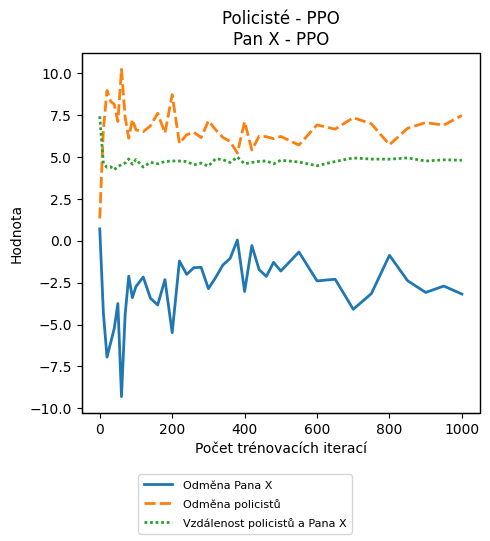
\includegraphics[width=1\textwidth]{obrazky-figures/graphs/cop_PPO_mrx_PPO}
      \caption{Graf simulace her, kde oba agenti volí akce dle modelu PPO}
      \label{fig:cop_ppo_mrx_ppo}
  \end{minipage}
  \caption{Srovnání PPO agenty s~agenty volící náhodné akce}
  \label{fig:srovnani_random_ppo}
  \end{figure}

Na srovnání~\ref{fig:srovnani_random_ppo} lze vidět, že na jak PPO, tak náhodný algoritmus udržují velice stabilní vzdálenost.
U~náhodného chování je to kvůli základní pravděpodobnosti, která musí být průměrně stejná.
U~grafu agentů PPO, to avšak vypovídá o~tom, že policisté dokáží stabilně odhadovat pozici Pana~X a přinejmenším se pohybovat v~jeho blízkém okolí.
Z~grafu\ref{fig:cop_ppo_mrx_ppo} lze pozorovat, že odměna policistů a Pana~X kolísá.
Frekvence tohoto kolísání se postupně jemně zmenšuje.
Z~toho odvozuji, že toto kolísání vypovídá o~tom, že se agenti postupně učí strategii protivníka a snaží se podle ní upravit svoji strategii, aby byli opět lepší.
Což značí, že se obě strategie pomalu přibližují k~optimu.
Předpokládám, že dalším trénováním, by se tento trend potvrdil.
Avšak k~tomu by bylo potřeba zapotřebí větší výpočetní výkon a spoustu času.
Ale jak lze vidět z~výsledků experimentu, i přes relativně malý počet trénovacích iterací se objevuje očekávané chování a rozdíl s~náhodným chováním je markantní.

\subsubsection*{Závěr experimentu pro algoritmus PPO}

Každá možná kombinace využití algoritmů pro policisty a Pana~X byla během experimentu testována celkově 2050$\times$.
Z~tohoto testování vzešly kromě grafů vývoje chování, také údaje zaznamenávající výsledky jednotlivých her.
Tyto výsledky byly zpracovány do tabulek, které zobrazují procentuální počet výher jednotlivých stran v~závislosti na použitém algoritmu.

\begin{figure}[H]
  \centering
  \begin{minipage}{.48\textwidth}
    \begin{table}[H]
    \centering
  \begin{tabular}{@{} c|c|c|c @{}}
  \headercell{\\Policisté} & \multicolumn{3}{c@{}}{Pan~X}\\
  \cmidrule(l){2-4}
  & \multicolumn{1}{c}{PPO}&\multicolumn{1}{c}{Random}&
  \multicolumn{1}{c}{DQN} \\ 
  \hline
  PPO                                    & 38 \% & 67 \% & 65 \% \\ \hline
  Random                                    & 11 \% & 20 \% & 18 \% \\ \hline
  DQN                                    & 10 \% & 17 \% & 19 \% \\ \hline
\end{tabular}
\caption{Zobrazuje procentuální počet výher policistů proti Pánovi~X s~vybraným algoritmem během experimentu}
\label{tab:train_experiment_police_wins}    
\end{table}  
\end{minipage}\hfill
  \begin{minipage}{.48\textwidth}
    \begin{table}[H]
    \centering
    \begin{tabular}{@{} c|c|c|c @{}}
      \headercell{\\Pan~X} & \multicolumn{3}{c@{}}{Policisté}\\
      \cmidrule(l){2-4}
      & \multicolumn{1}{c}{PPO}&\multicolumn{1}{c}{Random}&
      \multicolumn{1}{c}{DQN} \\
      \hline
      PPO                                    & 62 \% & 89 \% & 90 \% \\ \hline
      Random                                    & 33 \% & 80 \% & 83 \% \\ \hline
      DQN                                    & 35 \% & 82 \% & 81 \% \\ \hline
      \end{tabular}
      \caption{Zobrazuje procentuální počet výher Pana~X proti policistům s~vybraným algoritmem během experimentu}
      \label{tab:train_experiment_mrx_wins2}
    \end{table}
  \end{minipage}
  \end{figure}

Pokud zde opět porovnáme výsledky, kdy proti sobě hráli dva náhodní agenti a agenti trénovaní pomocí PPO, lze vidět, že agenti trénovaní pomocí PPO mají výrazně lepší výsledky.
\subsubsection{Ostatní výsledky}

\begin{figure}[H]
  \centering
  \begin{minipage}{.48\textwidth}
    \centering
    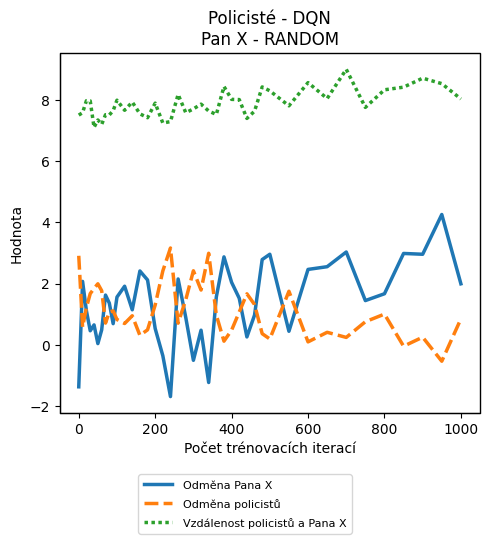
\includegraphics[width=1\textwidth]{obrazky-figures/graphs/cop_DQN_mrx_RANDOM}
    \caption{Graf simulace hry mezi policisty trénovanými pomocí DQN a Panem X volícím náhodné akce}
    \label{fig:cop_dqn_mrx_random}
  \end{minipage}\hfill
  \begin{minipage}{.48\textwidth}
    \centering
    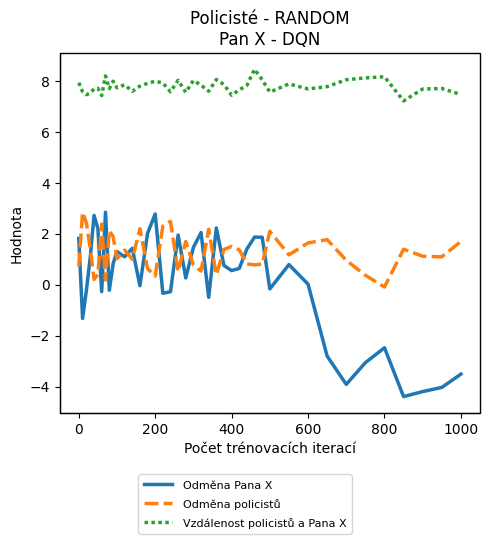
\includegraphics[width=1\textwidth]{obrazky-figures/graphs/cop_RANDOM_mrx_DQN}
      \caption{Graf simulace hry mezi Panem X trénovaným pomocí DQN a policisty volícími náhodné akce}
      \label{fig:cop_random_mrx_dqn}
  \end{minipage}
  \label{fig:srovnani_dqn}
  \end{figure}

Jak již jsem zmiňoval, výsledky trénování agentů pomocí algoritmu DQN bohužel nemají dobré výsledky.
Výsledné chování se velmi podobá náhodnému agentovi.
Z~předchozích prací je známo, že by algoritmus DQN měl mít znatelně lepší výsledky než náhodná metoda~\cite{Hrklova2023thesis}.
Algoritmus DQN je velice citlivý na hyperparametry a je možné, že bylo zvoleno nevhodné nastavení.
Potřebuje také mnohem více trénovacích iterací než PPO\@.
Je tedy možné, že 1000 iterací není dostatečné pro naučení dobré strategie pro algoritmus DQN\@.
Jelikož jsou ale trénovací iterace PPO časově náročnější než iterace DQN, nebylo možné sladit jejich počet.

\emph{Trénování z~tohoto experimentu poslouží jako základ pro další experiment, kde budou simulovány hry s~již natrénovanými agenty.}

\section{Experiment 2: Simulace hry s~již natrénovanými agenty}
\label{sec:experiment-2}

Tento experiment byl proveden za účelem ověření, zda jsou agenti trénováni pomocí algoritmu PPO schopni pochopit cíl hry a naučit se optimální strategii.
Porovnává, jestli již natrénované modely z~experimentu 1, výrazně liší od agenta který volí pouze náhodné akce a tím prokázat že se chová způsobem, který vede k~vítězství.

Pro ověření zkutečného výkonu agentů byly provedeny simulace hry mezi již natrénovanými agenty.
Ačkoli již předchozí experiment dokazuje, že agenti trénovaní pomocí algoritmu PPO jsou schopni pochopit cíl hry, je důležité získat skutečná data o~výkonu jednotlivých metod, bez zkreslených výsledků kvůli trénování.

Následující tabulky byly získány ze 10000 simulací pro každou kombinaci již natrénovaných algoritmů.

\begin{figure}[H]
  \centering
  \begin{minipage}{.48\textwidth}
    \begin{table}[H]
    \centering
  \begin{tabular}{@{} c|c|c|c @{}}
  \headercell{\\Policisté} & \multicolumn{3}{c@{}}{Pan~X}\\
  \cmidrule(l){2-4}
  & \multicolumn{1}{c}{PPO}&\multicolumn{1}{c}{Random}&
  \multicolumn{1}{c}{DQN} \\ 
  \hline
  PPO                                    & 26 \% & 72 \% & 64 \% \\ \hline
  Random                                    & 10 \% & 19 \% & 18 \% \\ \hline
  DQN                                    & 8 \% & 17 \% & 17 \% \\ \hline
\end{tabular}
\caption{Zobrazuje procentuální počet výher policistů proti Pánovi~X s~vybraným algoritmem}
\label{tab:simulation_experiment_police_wins}    
\end{table}  
\end{minipage}\hfill
  \begin{minipage}{.48\textwidth}
    \begin{table}[H]
    \centering
    \begin{tabular}{@{} c|c|c|c @{}}
      \headercell{\\Pan~X} & \multicolumn{3}{c@{}}{Policisté}\\
      \cmidrule(l){2-4}
      & \multicolumn{1}{c}{PPO}&\multicolumn{1}{c}{Random}&
      \multicolumn{1}{c}{DQN} \\
      \hline
      PPO                                    & 74 \% & 90 \% & 92 \% \\ \hline
      Random                                    & 28 \% & 81 \% & 82 \% \\ \hline
      DQN                                    & 36 \% & 82 \% & 83 \% \\ \hline
      \end{tabular}
      \caption{Zobrazuje procentuální počet výher Pana~X proti policistům s~vybraným algoritmem}
      \label{tab:train_experiment_mrx_wins}
    \end{table}
  \end{minipage}
  \end{figure}

Z~tabulky lze vyčíst, že policisté trénováni pomocí PPO vyhráli proti Pánovi~x s~náhodným chováním 72 \% her.
V~porovnání s~policisty volící náhodné akce je to výrazně lepší výsledek.
Ti proti Pánovi~x s~náhodným chováním vyhráli pouze 19 \% her.

Z~her vzešly také tyto informace:
\begin{itemize}
  \item Průměrná vzdálenost mezi Panem X a policisty (oba PPO): 4.779692656488397
  \item Průměrná vzdálenost mezi Panem X a policisty (oba náhodné chování): 7.631191103120987
  \item Průměrná vzdálenost mezi Panem X a policisty (oba DQN): 7.869671633109524
\end{itemize}

Z~tohoto experimentu lze tedy vyvodit, že agenti trénovaní pomocí algoritmu PPO prokázali, že se byli schopni naučit optimální strategii i ve hře s~neúplnou informací.

\chapter{Závěr}
\label{ch:zaver}

Provedené experimenty ukázaly, že algoritmus PPO je skutečně vhodný na hry s~neúplnou informací.
Jelikož policisté trénování pomocí PPO dokázali odhadovat přibližnou pozici Pana~X a měli mnohem větší úspěšnost než náhodní agenti.
Agenti se učili formou hraní proti sobě a dokázali pochopit koncept a cíl hry Scotland Yard.
Naučili se v~ní chovat optimálně, přestože začínali s~nulovým věděním o~prostředí.
Bylo příjemným překvapením, že již po pouhých 10 iterací trénování byli agenti schopni projevovat náznaky pochopení cíle hry.

\section*{Možná vylepšení}
\label{sec:mozna-vylepseni}

Bohužel se během experimentu nepovedlo separovat výslednou strategii od frameworku \texttt{Ray.Rlib} a extrahovat ji do podoby kde by již \texttt{Rlib} nebyl potřeba pro její využití.
Při spouštění hry se tedy načítá i celý framework \texttt{Ray.Rlib}, toto velmi zpomaluje načítání hry kdy prvotní načtení trvá několik sekund.
Toto a spoustu dalších potíží jsou důvody proč zvolení knihovny Ray.Rllib zpětně lituji.
Měl jsem spíše algoritmus PPO implementovat svépomocí s~využitím \texttt{Pytorch} či \texttt{Tensorflow}.
Nebo využít knihovnu \texttt{CleanRl} a učení více strategií naráz vyřešit jiným způsobem.

\medskip
Původním plánem bylo také realizovat možnost hraní hry mezi lidmy a agenty.
Tuto implementaci jsem, avšak přes problémy s~experimenty a algoritmem DQN nestihl dokončit.
Mám za to, že by tato možnost nadále prohloubila výsledky této studie o~zajímavé experimenty, kde by bylo možné sledovat jak si agent PPO vede proti lidskému protivníkovi.

\medskip
Agenti trénování pomocí algoritmu DQN měli velmi špatné výsledky.
Je vyloučeno, že by byla chyba v~prostředí, udělování odměn či v~pozorování jelikož se agenti trénovaní pomocí PPO učili za stejných podmínek a jejich výsledky byly dobré.
Je možné, že i přes hledání optimálních parametrů s~pomocí \texttt{Ray.Tune} byla zvolena nevhodná konfigurace.
Byť jsem s~těmito parametry dlouhosáhle experimentoval, nebylo dosaženo uspokojivých výsledků.
Navrhuji změnu stavového a akčního prostoru, aby byl kompatibilní s~verzemi studentů z~minulých let, kteří realizovali bakalářskou práci na podobné téma.
A~následně využít jejich implementaci pro další experimenty~\cite{Hrklova2023thesis}.

\medskip
Dále je zde možnost rozšířit hratelnost hry o~jednotlivé druhy dopravy a k~nim příslušící jízdenky.
Tím by výrazně vzrostla složitost hry a stavový prostor.
Jak ale ukázala práce OpenAI~\cite{Dota2}, algoritmus PPO nemá problém s~obrovským stavovým i akčním prostorem a naučit se i komplikované hry.



%===============================================================================

% Pro kompilaci po částech (viz projekt.tex) nutno odkomentovat
%\end{document}
